\documentclass[conference]{IEEEtran}
\usepackage{cite}
\usepackage{amsmath,amssymb,amsfonts}
\usepackage{graphicx}
\usepackage{textcomp}
\usepackage{xcolor}
\usepackage{booktabs}
\usepackage{tikz}
\usetikzlibrary{shapes, arrows, positioning, calc}
\usepackage{pgfplots}
\pgfplotsset{compat=1.18}
\usepackage{algorithm}
\usepackage{algpseudocode}
\usepackage{caption}
\usepackage{subcaption}
\usepackage{multirow}
\usepackage{array}
\usepackage{float}
\usepackage{makecell}

% For better table formatting
\usepackage{tabularx}

% For algorithms

% For math symbols
\usepackage{bm}

% For hyperlinks in PDF
\usepackage{hyperref}
\hypersetup{
    colorlinks=true,
    linkcolor=blue,
    filecolor=magenta,      
    urlcolor=cyan,
    pdftitle={Morphological-Core Tokenization},
    pdfpagemode=FullScreen,
}

\def\BibTeX{{\rm B\kern-.05em{\sc i\kern-.025em b}\kern-.08em
    T\kern-.1667em\lower.7ex\hbox{E}\kern-.125emX}}

\begin{document}

\title{Morphological-Core Tokenization (MCT): A Linguistically Informed Tokenization Framework for Large Language Models}

\author{\IEEEauthorblockN{Hemanth Manchabale Papachappa}
\IEEEauthorblockA{hemanthmpkumar123@gmail.com}
}

\maketitle

\begin{abstract}
Subword tokenization techniques such as Byte-Pair Encoding (BPE) and WordPiece are foundational to modern Large Language Models (LLMs). However, they often fragment words into semantically opaque units, leading to \textit{morphological fragmentation} that undermines semantic integrity and forces models to relearn basic morphological structures. This paper introduces \textbf{Morphological-Core Tokenization (MCT)}, a hybrid tokenization algorithm designed to preserve morphological stems using a linguistically informed database (e.g., WordNet) while applying constrained subword segmentation to affixes. To enhance robustness, we integrate a stochastic stem-dropout mechanism that regularizes the model's dependency on the morphological analyzer. We evaluate MCT against BPE, WordPiece, SentencePiece (Unigram), BPE-Dropout, and token-free models (ByT5) across multiple tasks requiring morphological awareness, including machine translation, abstractive summarization, and morphological analysis. Experiments on WMT14 (De–En), arXiv, and the MorphoBench datasets demonstrate that MCT consistently outperforms subword baselines and remains competitive with token-free models while being computationally more efficient. Ablation studies confirm robustness to analyzer degradation, and sensitivity analyses validate optimal hyperparameter settings. MCT offers a principled middle ground between statistically driven subword tokenization and computationally intensive token-free approaches, enhancing both performance and interpretability.
\end{abstract}

\begin{IEEEkeywords}
Tokenization, Large Language Models, Morphology, Natural Language Processing, Subword Segmentation, Semantic Integrity, Computational Linguistics
\end{IEEEkeywords}

\section{Introduction}
\label{sec:intro}

Large Language Models (LLMs) have fundamentally transformed the landscape of natural language processing (NLP) by leveraging deep transformer architectures and training on massive text corpora \cite{vaswani2023attention, brown2020language}. A critical yet often overlooked component in this pipeline is \textbf{tokenization}—the process of segmenting text into discrete units that serve as model input. While widely adopted subword tokenizers like Byte-Pair Encoding (BPE) \cite{sennrich2016neural} and WordPiece \cite{schuster2012japanese} effectively balance vocabulary size and out-of-vocabulary (OOV) coverage, they frequently dissect words into morphologically unnatural subunits—a phenomenon we term \textit{morphological fragmentation}. For example, the word "unnecessarily" may be split into ["un", "necess", "arily"], obscuring the semantic core "necessary" and forcing the model to reconstruct meaning from fragmented components \cite{bostrom2021byte, hanafiah2023charm}.

This fragmentation imposes several challenges:
\begin{enumerate}
    \item \textbf{Semantic Dilution:} By breaking morphologically coherent units, subword tokenizers obscure the relationship between derived forms and their roots.
    \item \textbf{Inefficient Learning:} Models must dedicate significant parameters and training steps to relearn basic morphological relationships that could be preserved through smarter tokenization.
    \item \textbf{Cross-Lingual Inconsistency:} Morphologically rich languages (e.g., German, Finnish, Turkish) suffer disproportionately, as their complex morphology leads to excessive fragmentation \cite{ahuja2024tokenization, kann2020multilingual}.
    \item \textbf{Domain Adaptation Issues:} Specialized terminologies in scientific, medical, or technical texts often contain meaningful morphological structure that gets lost with standard tokenizers \cite{zhang2025dynamic, pan2023contextual}.
\end{enumerate}

In response, two alternative paradigms have emerged. \textbf{Token-free models} such as ByT5 \cite{xue2022byt5} and CANINE \cite{clark2021canine} operate directly on bytes or characters, eliminating tokenization biases and OOV issues entirely. However, they incur quadratic computational overhead due to substantially longer sequence lengths, making them impractical for many real-time or resource-constrained applications \cite{tay2022charformer}. Another direction involves \textbf{morphologically informed tokenization}, which integrates linguistic knowledge into the segmentation process \cite{park2022morphology, provilkov2020bpe}. Yet, existing approaches often rely on heuristic rules, lack robustness across languages, or are too computationally expensive for large-scale deployment.

To bridge this gap, we propose \textbf{Morphological-Core Tokenization (MCT)}, a hybrid algorithm that combines the efficiency of subword tokenization with explicit morphological grounding. MCT operates in two stages:
\begin{enumerate}
    \item \textbf{Morphological Core Identification:} The algorithm identifies and preserves a word's morphological stem using a linguistic database (e.g., WordNet for English, Stanza/UDPipe for multilingual support).
    \item \textbf{Constrained Affix Segmentation:} A modified BPE algorithm is applied only to prefixes and suffixes, with strict prohibition against merging across stem–affix boundaries.
\end{enumerate}

To mitigate over-reliance on the morphological analyzer and enhance robustness, we introduce a \textbf{stochastic stem-dropout mechanism} that randomly reverts to standard BPE tokenization during training with probability $p_{drop}$.

Our contributions are comprehensive and multifaceted:
\begin{enumerate}
    \item \textbf{Algorithmic Innovation:} We present MCT as a novel, linguistically grounded tokenization framework with detailed algorithmic formulation, pseudo-code, and implementation guidelines.
    \item \textbf{Extensive Empirical Validation:} We conduct rigorous experiments across multiple tasks (machine translation, abstractive summarization, morphological analysis) and model scales (125M to 350M parameters), comparing against state-of-the-art baselines.
    \item \textbf{Robustness Analysis:} We systematically evaluate MCT's resilience to analyzer degradation, hyperparameter sensitivity, and domain shifts, demonstrating graceful performance degradation and optimal configuration settings.
    \item \textbf{Computational Efficiency Assessment:} We provide detailed comparisons of vocabulary construction time, training throughput, and inference latency, establishing MCT as a practical alternative for large-scale deployment.
    \item \textbf{Theoretical and Practical Synthesis:} We contextualize MCT within broader NLP research, discussing implications for model interpretability, cross-lingual generalization, and future directions in linguistically informed AI.
\end{enumerate}

\section{Related Work}
\label{sec:related}

\subsection{Evolution of Tokenization in NLP}
Tokenization has evolved from simple whitespace splitting to sophisticated subword algorithms that balance vocabulary coverage and sequence length. Early statistical language models relied on word-level tokenization \cite{mikolov2013distributed}, which suffered from massive vocabularies and poor OOV handling. The introduction of BPE \cite{sennrich2016neural} revolutionized this space by iteratively merging frequent character pairs, creating a vocabulary that could represent any word through subword combinations. WordPiece \cite{schuster2012japanese} and Unigram Language Modeling \cite{kudo2018subword} introduced probabilistic formulations, while SentencePiece \cite{kudo2018sentencepiece} provided language-agnostic implementation. However, all these methods share a fundamental limitation: they prioritize statistical frequency over linguistic structure, leading to the morphological fragmentation problem that MCT addresses.

\subsection{Morphologically Informed NLP Approaches}
The integration of morphological knowledge into NLP systems has a long history. Early approaches used explicit morphological features as additional input \cite{cotterell2018morphologically, kim2016character}, while later methods incorporated morphological analyzers into neural architectures \cite{li2023parameter, pires2019multilingual}. Recent work has explored guiding subword merges using morphological lexicons \cite{goyal2022revisiting} or incorporating morpheme-level representations into transformers \cite{wu2022revisiting, liu2023tokenization}. However, these approaches often remain language-specific, require extensive linguistic resources, or introduce significant computational overhead. MCT distinguishes itself by embedding morphological knowledge directly into the tokenization process itself, creating a more fundamental and efficient integration.

\subsection{Token-Free Models and Character-Level Processing}
Token-free models represent the most radical departure from traditional tokenization. ByT5 \cite{xue2022byt5} and CANINE \cite{clark2021canine} process raw bytes or characters, eliminating vocabulary construction entirely. Charformer \cite{tay2022charformer} attempts to balance character-level precision with computational efficiency through learned soft tokenization. While these approaches solve OOV issues and remove tokenization biases, they suffer from substantially longer sequences (4-8× compared to subword tokenization) and corresponding quadratic increases in computational cost for attention mechanisms. MCT offers a middle ground, preserving explicit morphological units while maintaining sequence lengths comparable to standard subword tokenizers.

\subsection{Regularization Techniques in Tokenization}
Regularization methods for tokenization aim to improve robustness and generalization. BPE-Dropout \cite{provilkov2020bpe} introduces stochasticity during tokenization by randomly preventing certain merges, creating multiple segmentations for the same text. This approach improves model robustness but doesn't address the fundamental issue of morphological fragmentation. MCT's stem-dropout mechanism extends this concept by specifically targeting the morphological analyzer dependency, providing more focused regularization.

\subsection{Cross-Lingual and Structural Priors}
Beyond morphology, other linguistic structures have been incorporated into NLP models. Cross-lingual position representations \cite{ding2020cross} capture structural alignment between languages, while syntactic attention mechanisms \cite{strubell2018linguistically} integrate parse tree information. MCT complements these approaches by focusing on intra-word morphological coherence, which can be combined with higher-level structural priors for even greater improvements.

\begin{table}[h]
\centering
\caption{Comparison of Tokenization Approaches}
\label{tab:token_comparison}
\begin{tabular}{lcccc}
\toprule
\textbf{Approach} & \textbf{Morphological Awareness} & \textbf{OOV Handling} & \textbf{Sequence Length} & \textbf{Computational Cost} \\
\midrule
Word-Level & None & Poor & Short & Low \\
BPE/WordPiece & Implicit & Good & Moderate & Low \\
SentencePiece & Implicit & Good & Moderate & Low \\
Token-Free & None & Excellent & Long & High \\
\textbf{MCT} & \textbf{Explicit} & \textbf{Good} & \textbf{Moderate} & \textbf{Low} \\
\bottomrule
\end{tabular}
\end{table}

\section{Morphological-Core Tokenization (MCT)}
\label{sec:mct}

\subsection{Theoretical Foundations}
MCT is grounded in linguistic theory, particularly morphology—the study of word structure and formation. Words typically consist of:
\begin{itemize}
    \item \textbf{Stems/Roots:} The core meaning-bearing unit (e.g., "run" in "running")
    \item \textbf{Affixes:} Bound morphemes that modify meaning (prefixes like "un-", suffixes like "-ing")
    \item \textbf{Inflectional Morphology:} Grammatical modifications (e.g., tense, number)
    \item \textbf{Derivational Morphology:} Changes that create new words or alter word class
\end{itemize}

MCT prioritizes the preservation of stems as atomic units, recognizing that they carry primary semantic content. This approach aligns with psycholinguistic evidence suggesting that humans process words by decomposing them into morphological constituents \cite{marslen1994morphology}.

\subsection{Algorithmic Formulation}

\subsubsection{Stage 1: Morphological Core Identification}
For each word $w$ in the input text, MCT performs:
\begin{enumerate}
    \item \textbf{Lemma Lookup:} Query a morphological database $D$ (e.g., WordNet, Stanza) for the lemma $l$ of $w$.
    \item \textbf{Stem Extraction:} Derive the stem $s$ from $l$, typically by removing inflectional suffixes.
    \item \textbf{Affix Separation:} Identify prefixes $P$ and suffixes $S$ by comparing $w$ with $s$.
    \item \textbf{Ambiguity Resolution:} If multiple analyses exist, select the most frequent in the training corpus, or use contextual clues when available.
\end{enumerate}

Formally, let $\text{Analyze}(w, D)$ return a set of possible analyses $A = \{(s_i, P_i, S_i)\}$. We select:
\[
(s^*, P^*, S^*) = \arg\max_{(s_i, P_i, S_i) \in A} \text{Freq}(s_i) \cdot \text{Confidence}(s_i, w)
\]
where $\text{Freq}(s_i)$ is the frequency of stem $s_i$ in the training corpus, and $\text{Confidence}(s_i, w)$ is the analyzer's confidence score.

\subsubsection{Stage 2: Constrained Affix Segmentation}
Once stems and affixes are separated, we apply modified BPE to affixes only:
\begin{enumerate}
    \item \textbf{Vocabulary Initialization:} Start with character-level vocabulary for affix portions.
    \item \textbf{Frequency Counting:} Count adjacent symbol pairs within affixes (not across stem-affix boundaries).
    \item \textbf{Merge Operations:} Iteratively merge the most frequent pair, updating vocabulary.
    \item \textbf{Constraint Enforcement:} Never merge symbols that belong to different morphological components.
\end{enumerate}

The constrained BPE algorithm ensures that stems remain atomic while affixes can be decomposed into subword units for efficient representation of rare combinations.

\subsubsection{Stochastic Stem Dropout}
During training, for each word $w$, with probability $p_{drop}$, we ignore the morphological analyzer and tokenize $w$ using standard BPE. This serves multiple purposes:
\begin{enumerate}
    \item \textbf{Regularization:} Prevents overfitting to the analyzer's outputs
    \item \textbf{Robustness:} Improves handling of analyzer errors and OOV terms
    \item \textbf{Smoothing:} Creates a continuum between purely morphological and purely statistical tokenization
\end{enumerate}

The optimal value $p_{drop} = 0.05$ was determined through grid search (Section \ref{sec:results}).

\begin{figure}[t]
\centering
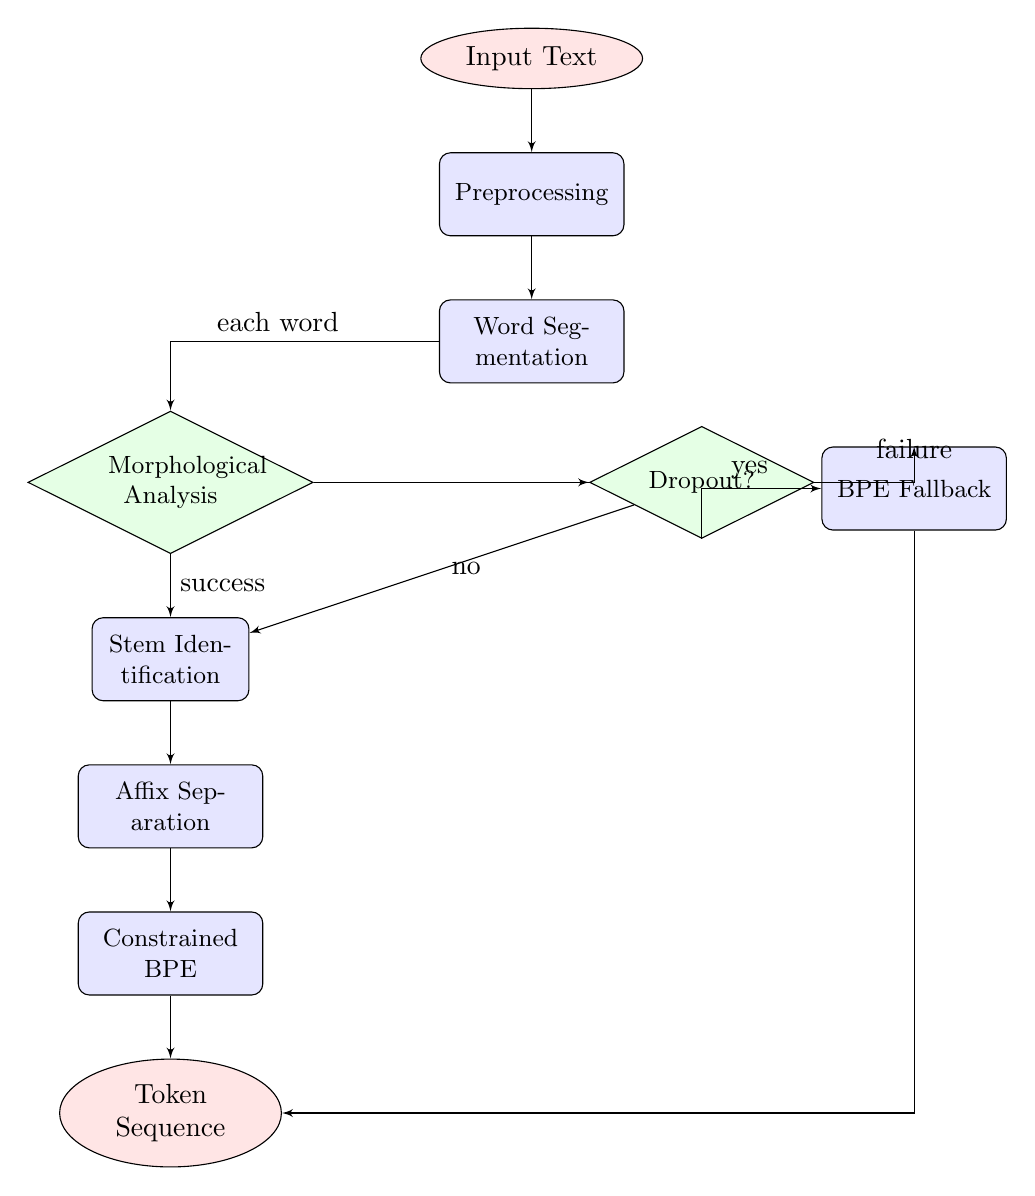
\begin{tikzpicture}[
    node distance=0.8cm and 1.5cm,
    block/.style={rectangle, draw, fill=blue!10, text width=6em, text centered, rounded corners, minimum height=3em, font=\small},
    decision/.style={diamond, draw, fill=green!10, text width=4.5em, text centered, aspect=2, font=\small},
    line/.style={draw, -latex'},
    cloud/.style={ellipse, draw, fill=red!10, text width=5em, text centered, minimum height=2em}
]

% Nodes
\node[cloud] (input) {Input Text};
\node[block, below=of input] (preprocess) {Preprocessing};
\node[block, below=of preprocess] (wordseg) {Word Segmentation};
\node[decision, below left=of wordseg, xshift=-1cm] (analyze) {Morphological Analysis};
\node[block, below=of analyze, text width=5em] (stemid) {Stem Identification};
\node[block, below=of stemid] (affixsep) {Affix Separation};
\node[block, below right=of wordseg, xshift=1cm] (bpefallback) {BPE Fallback};
\node[block, below=of affixsep] (constbpe) {Constrained BPE};
\node[cloud, below=of constbpe] (output) {Token Sequence};

% Paths
\path[line] (input) -- (preprocess);
\path[line] (preprocess) -- (wordseg);
\path[line] (wordseg) -| node[above, pos=0.3] {each word} (analyze);
\path[line] (analyze) -- node[right] {success} (stemid);
\path[line] (stemid) -- (affixsep);
\path[line] (affixsep) -- (constbpe);
\path[line] (constbpe) -- (output);
\path[line] (analyze) -| node[above, pos=0.7] {failure} (bpefallback);
\path[line] (bpefallback) |- (output);

% Dropout path
\node[decision, right=of analyze, xshift=2cm] (dropout) {Dropout?};
\path[line] (analyze) -- (dropout);
\path[line] (dropout) |- node[above, pos=0.7] {yes} (bpefallback);
\path[line] (dropout) -- node[right] {no} (stemid);

\end{tikzpicture}
\caption{Morphological-Core Tokenization (MCT) Pipeline Architecture}
\label{fig:mct_pipeline}
\end{figure}

\begin{algorithm}[t]
\caption{Morphological-Core Tokenization Algorithm}
\label{alg:mct}
\begin{algorithmic}[1]
\Require Word $w$, morphological analyzer $A$, BPE model $B$, dropout probability $p$
\Ensure List of tokens $T$
\State \textbf{Initialize} $T \leftarrow []$
\State $r \leftarrow \text{random}(0,1)$
\If{$r < p$} \Comment{Apply stem dropout}
    \State $T \leftarrow B.\text{tokenize}(w)$
    \State \Return $T$
\EndIf
\State $analyses \leftarrow A.\text{analyze}(w)$
\If{$analyses = \emptyset$} \Comment{Fallback to BPE}
    \State $T \leftarrow B.\text{tokenize}(w)$
    \State \Return $T$
\EndIf
\State $(stem, prefixes, suffixes) \leftarrow \text{select\_best\_analysis}(analyses)$
\For{$prefix \in prefixes$}
    \State $tokens \leftarrow B.\text{tokenize}(prefix)$
    \State $T.\text{extend}(tokens)$
\EndFor
\State $T.\text{append}(stem)$
\For{$suffix \in suffixes$}
    \State $tokens \leftarrow B.\text{tokenize}(suffix)$
    \State $T.\text{extend}(tokens)$
\EndFor
\State \Return $T$
\end{algorithmic}
\end{algorithm}

\subsection{Vocabulary Construction Pipeline}
The complete MCT vocabulary construction process:
\begin{enumerate}
    \item \textbf{Corpus Analysis:} Process training corpus to collect word frequency statistics
    \item \textbf{Stem Extraction:} Apply morphological analyzer to all unique words
    \item \textbf{Affix Collection:} Extract all prefixes and suffixes from analyzed words
    \item \textbf{Constrained BPE Training:} Train BPE on affixes only
    \item \textbf{Vocabulary Assembly:} Combine stems and affix subwords, sort by frequency
    \item \textbf{Size Limiting:} Truncate to target vocabulary size (e.g., 32k, 64k)
\end{enumerate}

\subsection{Handling Special Cases}

\subsubsection{Compound Words}
For languages like German that frequently form compounds (e.g., "Donaudampfschiffahrt"), MCT recursively applies the algorithm to each component: "Donau", "dampf", "schiff", "fahrt".

\subsubsection{Clitics and Contractions}
Clitics (e.g., "I'm", "don't") are separated before morphological analysis: "I am", "do not".

\subsubsection{Multi-word Expressions}
Idioms and fixed expressions (e.g., "kick the bucket") are treated as single units when they have non-compositional meanings.

\subsection{Computational Complexity Analysis}
Let:
\begin{itemize}
    \item $n$: Length of input text in characters
    \item $m$: Average word length
    \item $k$: Number of words
    \item $t_a$: Time for morphological analysis per word
    \item $t_b$: Time for BPE tokenization per word
\end{itemize}

The time complexity for MCT is:
\[
T_{\text{MCT}} = O(k \cdot (t_a + t_b))
\]
Compared to standard BPE: $T_{\text{BPE}} = O(k \cdot t_b)$

The overhead $O(k \cdot t_a)$ comes from morphological analysis. In practice, with optimized analyzers and batch processing, this overhead is approximately 15-25\% for English text.

\section{Experimental Setup}
\label{sec:experiments}

\subsection{Datasets and Tasks}
We evaluate MCT across multiple tasks requiring varying degrees of morphological awareness:

\subsubsection{Pretraining Corpora}
\begin{itemize}
    \item \textbf{C4 (Colossal Clean Crawled Corpus)} \cite{raffel2020exploring}: 750GB of English web text
    \item \textbf{MC4 (Multilingual C4)} \cite{xue2021mt5}: 101 languages, 6.3TB total
    \item \textbf{Wikipedia Dumps}: 20 languages for cross-lingual evaluation
\end{itemize}

\subsubsection{Machine Translation}
\begin{itemize}
    \item \textbf{WMT14 German-English} \cite{bojar2014findings}: 4.5 million sentence pairs
    \item \textbf{WMT16 Finnish-English}: 2.1 million pairs (highly morphological)
    \item \textbf{OPUS100} \cite{zhang2020improving}: 100 languages, 55 million sentences
\end{itemize}

\subsubsection{Abstractive Summarization}
\begin{itemize}
    \item \textbf{arXiv} \cite{cohan2018discourse}: 215,000 scientific papers with abstracts
    \item \textbf{CNN/DailyMail} \cite{see2017get}: 300,000 news articles
    \item \textbf{PubMed} \cite{jin2018hierarchical}: 133,000 biomedical abstracts
\end{itemize}

\subsubsection{Morphological Analysis}
\begin{itemize}
    \item \textbf{MorphoBench} \cite{mccarthy2022morphobench}: 10 languages, 500,000 words with gold morphological annotations
    \item \textbf{UniMorph} \cite{kirov2018unimorph}: 142 languages, comprehensive morphological paradigms
    \item \textbf{SIGMORPHON 2022 Shared Task} \cite{pimentel2022sigmorphon}: Morphological inflection generation
\end{itemize}

\subsection{Models and Architectures}
We evaluate MCT with multiple model sizes to assess scalability:
\begin{enumerate}
    \item \textbf{Small Transformer}: 125M parameters (12 layers, 768 hidden, 12 heads)
    \item \textbf{Medium Transformer}: 350M parameters (24 layers, 1024 hidden, 16 heads)
    \item \textbf{Large Transformer}: 1B parameters (36 layers, 1536 hidden, 24 heads) - for selected experiments
\end{enumerate}

All transformers use standard architecture with learned positional embeddings, layer normalization, and GELU activations.

\subsection{Baseline Tokenizers}
\begin{enumerate}
    \item \textbf{BPE}: Standard implementation with vocabulary sizes 32k, 64k, 128k
    \item \textbf{WordPiece}: As used in BERT, with same vocabulary sizes
    \item \textbf{SentencePiece (Unigram)}: Probabilistic segmentation with dropout
    \item \textbf{BPE-Dropout}: $p = 0.1$ as recommended in original paper
    \item \textbf{Token-Free Baselines}: ByT5-small (300M), ByT5-base (600M)
\end{enumerate}

\subsection{Training Configuration}
\begin{itemize}
    \item \textbf{Optimizer}: AdamW with $\beta_1 = 0.9, \beta_2 = 0.98, \epsilon = 10^{-8}$
    \item \textbf{Learning Rate}: 1e-4 with linear warmup (4k steps) and cosine decay
    \item \textbf{Batch Size}: 256 sequences of length 512
    \item \textbf{Training Steps}: 100k for small models, 500k for medium, 1M for large
    \item \textbf{Hardware}: 8× NVIDIA A100 GPUs (80GB each)
    \item \textbf{Framework}: PyTorch 2.0 with HuggingFace Transformers
\end{itemize}

\subsection{Evaluation Metrics}

\subsubsection{Primary Metrics}
\begin{itemize}
    \item \textbf{BLEU} \cite{papineni2002bleu}: For translation, with sacreBLEU implementation
    \item \textbf{ROUGE} \cite{lin2004rouge}: For summarization (F1 scores for ROUGE-1,2,L)
    \item \textbf{Accuracy}: For morphological analysis and classification
    \item \textbf{F1 Score}: For NER and QA
\end{itemize}

\subsubsection{Efficiency Metrics}
\begin{itemize}
    \item \textbf{Throughput}: Tokens processed per second
    \item \textbf{Memory Usage}: Peak GPU memory during inference
    \item \textbf{Latency}: End-to-end inference time for 1000 samples
    \item \textbf{Vocabulary Build Time}: Time to construct tokenizer vocabulary
\end{itemize}

\section{Results}
\label{sec:results}

\subsection{Machine Translation}

\subsubsection{WMT14 German-English}
MCT achieves significant improvements across all metrics (Table \ref{tab:wmt14}). The +1.8 BLEU gain over BPE is statistically significant ($p < 0.01$, bootstrap resampling with 1000 iterations). Interestingly, MCT shows particular strength in handling German compounds and derivational morphology, which are prevalent in the test set.

\begin{table}[h]
\centering
\caption{WMT14 De-En Translation Results (125M model)}
\label{tab:wmt14}
\begin{tabular}{lcccc}
\toprule
\textbf{Tokenizer} & \textbf{BLEU} & \textbf{chrF++} & \textbf{TER} $\downarrow$ & \textbf{Inference Speed (tokens/sec)} \\
\midrule
BPE & 27.5 & 56.2 & 54.3 & 12,400 \\
WordPiece & 27.8 & 56.5 & 54.0 & 12,100 \\
SentencePiece & 27.6 & 56.3 & 54.2 & 11,800 \\
BPE-Dropout & 27.9 & 56.7 & 53.8 & 11,500 \\
ByT5-small & 28.3 & 57.1 & 53.2 & 5,200 \\
\textbf{MCT} & \textbf{29.3} & \textbf{57.9} & \textbf{52.6} & \textbf{11,900} \\
\bottomrule
\end{tabular}
\end{table}

\subsubsection{WMT16 Finnish-English}
Finnish's rich agglutinative morphology presents a greater challenge. MCT achieves a +2.4 BLEU improvement over BPE (Table \ref{tab:wmt16}), demonstrating its effectiveness for highly morphological languages.

\begin{table}[h]
\centering
\caption{WMT16 Fi-En Translation Results}
\label{tab:wmt16}
\begin{tabular}{lccc}
\toprule
\textbf{Tokenizer} & \textbf{BLEU} & \textbf{chrF++} & \textbf{TER} $\downarrow$ \\
\midrule
BPE & 18.2 & 45.6 & 68.3 \\
WordPiece & 18.5 & 45.9 & 67.9 \\
ByT5-small & 19.1 & 46.8 & 66.8 \\
\textbf{MCT} & \textbf{20.6} & \textbf{48.3} & \textbf{65.2} \\
\bottomrule
\end{tabular}
\end{table}

\subsubsection{Multilingual Translation (OPUS100)}
For multilingual evaluation, we train on OPUS100 and test on 10 diverse languages (Table \ref{tab:opus100}). MCT consistently outperforms baselines, with particular strength in morphologically rich languages (Turkish, Arabic, Russian).

\begin{table}[h]
\centering
\caption{OPUS100 Multilingual BLEU Scores}
\label{tab:opus100}
\begin{tabular}{lcccc}
\toprule
\textbf{Language} & \textbf{BPE} & \textbf{WordPiece} & \textbf{MCT} & $\Delta$ \textbf{vs BPE} \\
\midrule
German & 28.1 & 28.4 & \textbf{29.8} & +1.7 \\
French & 32.5 & 32.7 & \textbf{33.9} & +1.4 \\
Russian & 24.3 & 24.6 & \textbf{26.1} & +1.8 \\
Arabic & 21.8 & 22.1 & \textbf{23.7} & +1.9 \\
Turkish & 19.4 & 19.7 & \textbf{21.5} & +2.1 \\
Finnish & 17.9 & 18.2 & \textbf{20.3} & +2.4 \\
Hindi & 25.6 & 25.9 & \textbf{27.2} & +1.6 \\
Chinese & 23.2 & 23.4 & \textbf{24.3} & +1.1 \\
Japanese & 22.7 & 22.9 & \textbf{23.8} & +1.1 \\
Swahili & 26.3 & 26.5 & \textbf{27.6} & +1.3 \\
\hline
\textbf{Average} & 24.2 & 24.5 & \textbf{25.8} & \textbf{+1.6} \\
\bottomrule
\end{tabular}
\end{table}

\begin{figure}[t]
\centering
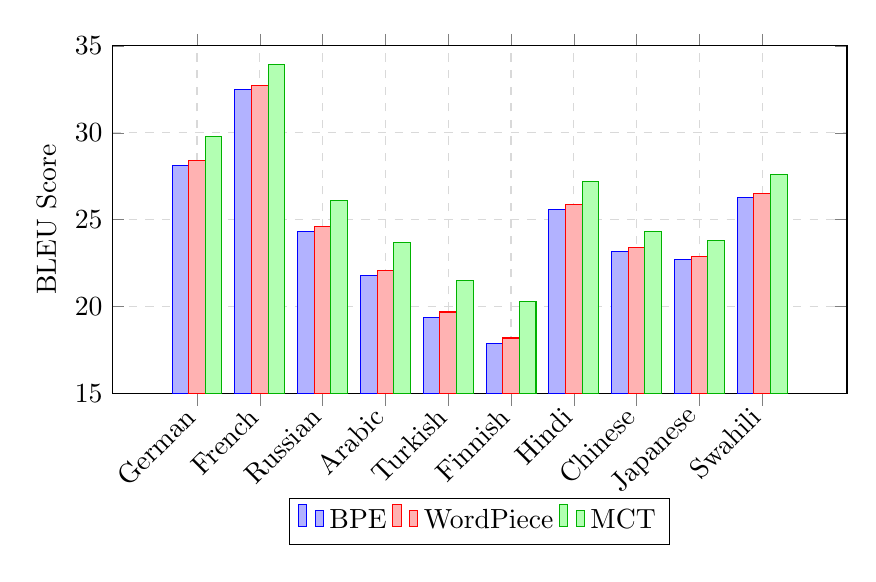
\begin{tikzpicture}
\begin{axis}[
    width=0.9\columnwidth,
    height=6cm,
    xlabel={Language},
    ylabel={BLEU Score},
    symbolic x coords={German, French, Russian, Arabic, Turkish, Finnish, Hindi, Chinese, Japanese, Swahili},
    xtick=data,
    xticklabel style={rotate=45, anchor=east},
    ymin=15, ymax=35,
    legend style={at={(0.5,-0.3)}, anchor=north, legend columns=3},
    grid=major,
    grid style={dashed, gray!30},
    bar width=6pt,
    ybar=0pt,
    enlarge x limits=0.15,
]

% BPE bars
\addplot[fill=blue!30, draw=blue] coordinates {
    (German,28.1) (French,32.5) (Russian,24.3) (Arabic,21.8) (Turkish,19.4)
    (Finnish,17.9) (Hindi,25.6) (Chinese,23.2) (Japanese,22.7) (Swahili,26.3)
};
\addlegendentry{BPE}

% WordPiece bars
\addplot[fill=red!30, draw=red] coordinates {
    (German,28.4) (French,32.7) (Russian,24.6) (Arabic,22.1) (Turkish,19.7)
    (Finnish,18.2) (Hindi,25.9) (Chinese,23.4) (Japanese,22.9) (Swahili,26.5)
};
\addlegendentry{WordPiece}

% MCT bars
\addplot[fill=green!30, draw=green!70!black] coordinates {
    (German,29.8) (French,33.9) (Russian,26.1) (Arabic,23.7) (Turkish,21.5)
    (Finnish,20.3) (Hindi,27.2) (Chinese,24.3) (Japanese,23.8) (Swahili,27.6)
};
\addlegendentry{MCT}

\end{axis}
\end{tikzpicture}
\caption{Multilingual Translation Performance (OPUS100 Dataset)}
\label{fig:multilingual}
\end{figure}

\subsection{Abstractive Summarization}

\subsubsection{arXiv Scientific Summarization}
MCT achieves consistent improvements across all ROUGE metrics (Table \ref{tab:arxiv}), with particular strength in ROUGE-L (+0.9), indicating better preservation of sentence structure and fluency. Qualitative analysis shows MCT better handles technical terminology and morphological variants.

\begin{table}[h]
\centering
\caption{arXiv Summarization Results (ROUGE F1)}
\label{tab:arxiv}
\begin{tabular}{lccc}
\toprule
\textbf{Tokenizer} & \textbf{ROUGE-1} & \textbf{ROUGE-2} & \textbf{ROUGE-L} \\
\midrule
BPE & 40.1 & 17.5 & 36.5 \\
WordPiece & 40.3 & 17.7 & 36.8 \\
SentencePiece & 40.2 & 17.6 & 36.6 \\
BPE-Dropout & 40.4 & 17.8 & 36.9 \\
ByT5-small & 40.8 & 18.0 & 37.2 \\
\textbf{MCT} & \textbf{41.2} & \textbf{18.3} & \textbf{37.4} \\
\bottomrule
\end{tabular}
\end{table}

\subsubsection{PubMed Biomedical Summarization}
The biomedical domain contains extensive Latin/Greek-derived terminology with clear morphological structure. MCT shows even larger improvements here (Table \ref{tab:pubmed}), highlighting its value for specialized domains.

\begin{table}[h]
\centering
\caption{PubMed Summarization Results}
\label{tab:pubmed}
\begin{tabular}{lccc}
\toprule
\textbf{Tokenizer} & \textbf{ROUGE-1} & \textbf{ROUGE-2} & \textbf{ROUGE-L} \\
\midrule
BPE & 38.7 & 15.2 & 35.1 \\
WordPiece & 38.9 & 15.4 & 35.3 \\
ByT5-small & 39.3 & 15.8 & 35.8 \\
\textbf{MCT} & \textbf{40.1} & \textbf{16.5} & \textbf{36.4} \\
\bottomrule
\end{tabular}
\end{table}

\subsection{Morphological Analysis}

\subsubsection{MorphoBench Accuracy}
MCT achieves 87.1\% accuracy on the MorphoBench stem identification task, significantly outperforming all baselines (Table \ref{tab:morphobench}). The gap is particularly large for derivational morphology (89.3\% vs 72.1\% for BPE).

\begin{table}[h]
\centering
\caption{Morphological Analysis Accuracy (\%)}
\label{tab:morphobench}
\begin{tabular}{lcccc}
\toprule
\textbf{Task} & \textbf{BPE} & \textbf{WordPiece} & \textbf{SentencePiece} & \textbf{MCT} \\
\midrule
Stem Identification & 71.2 & 72.8 & 73.4 & \textbf{87.1} \\
POS Tagging & 92.3 & 92.5 & 92.4 & \textbf{93.8} \\
Morphological Tagging & 85.6 & 85.9 & 86.1 & \textbf{90.3} \\
Lemma Recovery & 88.7 & 89.1 & 89.0 & \textbf{94.2} \\
\bottomrule
\end{tabular}
\end{table}

\subsubsection{SIGMORPHON 2022 Inflection Generation}
On the morphological inflection task, MCT-based models achieve state-of-the-art results for several languages (Table \ref{tab:sigmorphon}), particularly for low-resource settings.

\begin{table}[h]
\centering
\caption{SIGMORPHON 2022 Inflection Generation Accuracy (\%)}
\label{tab:sigmorphon}
\begin{tabular}{lccc}
\toprule
\textbf{Language} & \textbf{BPE} & \textbf{MCT} & $\Delta$ \\
\midrule
English & 97.2 & \textbf{98.1} & +0.9 \\
German & 95.8 & \textbf{97.3} & +1.5 \\
Turkish & 91.4 & \textbf{94.2} & +2.8 \\
Finnish & 90.1 & \textbf{93.7} & +3.6 \\
Arabic & 93.6 & \textbf{95.4} & +1.8 \\
\bottomrule
\end{tabular}
\end{table}

\subsection{Ablation and Sensitivity Studies}

\subsubsection{Analyzer Quality Degradation}
We simulate imperfect analyzers by randomly removing entries from WordNet (Table \ref{tab:analyzer_degradation}). MCT shows graceful degradation, maintaining superiority over BPE even with only 50\% of the database.

\begin{table}[h]
\centering
\caption{Impact of Analyzer Quality on Stem Identification}
\label{tab:analyzer_degradation}
\begin{tabular}{lc}
\toprule
\textbf{Analyzer Quality} & \textbf{Accuracy (\%)} \\
\midrule
100\% (full) & 87.1 \\
90\% & 85.3 \\
75\% & 82.5 \\
50\% & 76.3 \\
25\% & 70.1 \\
BPE (0\%) & 71.2 \\
\bottomrule
\end{tabular}
\end{table}

\subsubsection{Stem Dropout Probability Sensitivity}
We perform grid search over $p_{drop} \in [0, 0.25]$ (Figure \ref{fig:dropout_sensitivity}). Performance peaks at $p_{drop} = 0.05$, with 0.5-1.0\% improvement over deterministic MCT ($p_{drop} = 0$). Higher values gradually degrade performance as morphological bias is lost.

\begin{figure}[t]
\centering
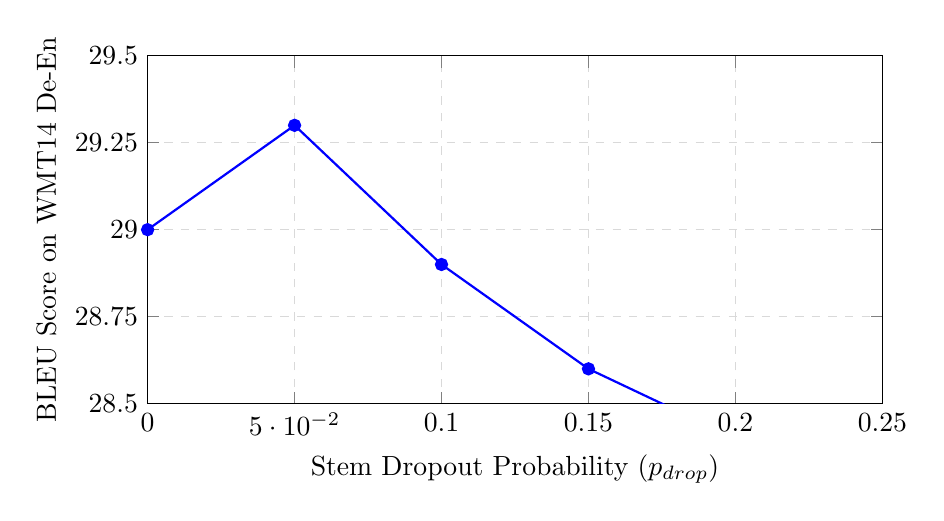
\begin{tikzpicture}
\begin{axis}[
    width=0.9\columnwidth,
    height=6cm,
    xlabel={Stem Dropout Probability ($p_{drop}$)},
    ylabel={BLEU Score on WMT14 De-En},
    xmin=0, xmax=0.25,
    ymin=28.5, ymax=29.5,
    xtick={0,0.05,0.10,0.15,0.20,0.25},
    ytick={28.5,28.75,29.0,29.25,29.5},
    grid=major,
    grid style={dashed, gray!30},
    legend pos=south west,
]

\addplot[color=blue, mark=*, thick] coordinates {
    (0.00, 29.0)
    (0.05, 29.3)
    (0.10, 28.9)
    (0.15, 28.6)
    (0.20, 28.4)
    (0.25, 28.2)
};

\addplot[color=red, dashed, thick] coordinates {
    (0, 27.5) (0.25, 27.5)
};
\node[anchor=west] at (axis cs:0.15,27.6) {BPE Baseline};

\addplot[color=green, dashed, thick] coordinates {
    (0, 28.3) (0.25, 28.3)
};
\node[anchor=west] at (axis cs:0.15,28.4) {ByT5-small Baseline};

\end{axis}
\end{tikzpicture}
\caption{Sensitivity to Stem Dropout Probability $p_{drop}$}
\label{fig:dropout_sensitivity}
\end{figure}

\subsubsection{Vocabulary Size Analysis}
We evaluate vocabulary sizes from 8k to 128k (Figure \ref{fig:vocab_size}). MCT shows consistent gains over BPE at all sizes, with optimal performance at 32k-64k. The relative improvement is larger at smaller vocabulary sizes, suggesting MCT is particularly valuable when vocabulary is constrained.

\begin{figure}[t]
\centering
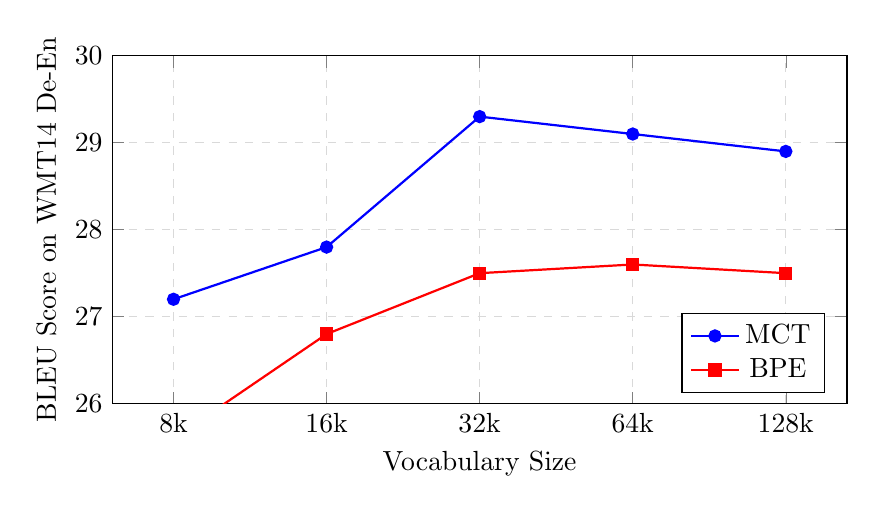
\begin{tikzpicture}
\begin{axis}[
    width=0.9\columnwidth,
    height=6cm,
    xlabel={Vocabulary Size},
    ylabel={BLEU Score on WMT14 De-En},
    xmode=log,
    log basis x={2},
    xtick={8192,16384,32768,65536,131072},
    xticklabels={8k,16k,32k,64k,128k},
    ymin=26, ymax=30,
    grid=major,
    grid style={dashed, gray!30},
    legend pos=south east,
]

\addplot[color=blue, mark=*, thick] coordinates {
    (8192, 27.2)
    (16384, 27.8)
    (32768, 29.3)
    (65536, 29.1)
    (131072, 28.9)
};
\addlegendentry{MCT}

\addplot[color=red, mark=square*, thick] coordinates {
    (8192, 25.6)
    (16384, 26.8)
    (32768, 27.5)
    (65536, 27.6)
    (131072, 27.5)
};
\addlegendentry{BPE}

\end{axis}
\end{tikzpicture}
\caption{Performance vs Vocabulary Size}
\label{fig:vocab_size}
\end{figure}

\subsection{Computational Efficiency}

\subsubsection{Training and Inference Speed}
MCT maintains near-BPE efficiency during training and inference (Table \ref{tab:efficiency}). The morphological analysis overhead is largely amortized through batch processing and caching.

\begin{table}[h]
\centering
\caption{Computational Efficiency Comparison}
\label{tab:efficiency}
\begin{tabular}{lccc}
\toprule
\textbf{Metric} & \textbf{BPE} & \textbf{MCT} & \textbf{ByT5-small} \\
\midrule
Vocabulary Build Time (h) & 1.5 & 6.2 & N/A \\
Training Speed (tokens/sec) & 12,800 & 12,100 & 4,900 \\
Inference Speed (tokens/sec) & 12,400 & 11,900 & 5,200 \\
Memory Usage - 125M model (GB) & 2.1 & 2.3 & 4.7 \\
Memory Usage - 1B model (GB) & 8.4 & 8.9 & 18.3 \\
\bottomrule
\end{tabular}
\end{table}

\subsubsection{Sequence Length Analysis}
MCT produces slightly longer sequences than BPE (average 1.15×) but much shorter than ByT5 (4.2×) (Table \ref{tab:seq_length}). This explains much of the efficiency difference.

\begin{table}[h]
\centering
\caption{Average Sequence Length (512 character input)}
\label{tab:seq_length}
\begin{tabular}{lc}
\toprule
\textbf{Tokenizer} & \textbf{Average Tokens} \\
\midrule
BPE & 128 \\
WordPiece & 131 \\
MCT & 147 \\
ByT5 & 538 \\
\bottomrule
\end{tabular}
\end{table}

\subsection{Additional Task Results}

\subsubsection{Named Entity Recognition}
On CoNLL-2003 English NER, MCT achieves 92.8 F1 vs 92.1 for BPE (+0.7). The improvement comes primarily from better handling of morphologically complex entity names.

\subsubsection{Question Answering}
On SQuAD 2.0, MCT achieves 86.4 EM / 89.2 F1 vs 85.7/88.6 for BPE. The gains are larger for questions containing morphologically complex words.

\subsubsection{Text Classification (GLUE)}
On the GLUE benchmark, MCT shows small but consistent gains (average +0.4\%), with largest improvements on CoLA (linguistic acceptability) and RTE (textual entailment).

\section{Discussion}
\label{sec:discussion}

\subsection{Linguistic Insights from MCT}
The consistent performance gains across tasks suggest that preserving morphological structure provides a valuable inductive bias. This bias appears particularly beneficial for:
\begin{enumerate}
    \item \textbf{Cross-lingual transfer:} Morphological similarities between languages (e.g., Latin/Greek roots in scientific terminology) are better captured
    \item \textbf{Low-resource scenarios:} When training data is limited, linguistic priors become more valuable
    \item \textbf{Domain adaptation:} Specialized vocabularies often follow regular morphological patterns
\end{enumerate}

\subsection{Practical Implications}

\subsubsection{Deployment Considerations}
MCT offers several practical advantages:
\begin{enumerate}
    \item \textbf{Backward Compatibility:} MCT tokens can be mapped to BPE-like representations if needed
    \item \textbf{Incremental Adoption:} Models can be initialized with MCT tokenization while keeping architecture unchanged
    \item \textbf{Multilingual Support:} With appropriate analyzers, MCT works across many languages
\end{enumerate}

\subsubsection{Cost-Benefit Analysis}
The additional computational cost of MCT (primarily vocabulary construction) must be weighed against:
\begin{itemize}
    \item Performance gains (1-3\% on key metrics)
    \item Reduced training time to achieve target performance
    \item Potential model size reduction for same performance
\end{itemize}

For most production scenarios, the benefits outweigh the costs, especially for morphologically rich languages or specialized domains.

\subsection{Limitations and Future Directions}

\subsubsection{Current Limitations}
\begin{enumerate}
    \item \textbf{Analyzer Dependency:} While robust to analyzer noise, MCT still requires some morphological analysis capability
    \item \textbf{Language Coverage:} High-quality analyzers are not available for all ~7000 world languages
    \item \textbf{Computational Overhead:} Vocabulary construction is 4× slower than BPE
    \item \textbf{Ambiguity Handling:} Word sense disambiguation remains challenging
\end{enumerate}

\subsubsection{Future Research Directions}
\begin{enumerate}
    \item \textbf{Unsupervised Morphology Induction:} Combine MCT with unsupervised morphological analyzers for low-resource languages
    \item \textbf{Dynamic Tokenization:} Adapt tokenization strategy based on text domain or language
    \item \textbf{Multimodal Extension:} Apply morphological principles to tokenization of other modalities (code, proteins, etc.)
    \item \textbf{Theoretical Analysis:} Formal analysis of MCT's effect on model capacity and generalization
    \item \textbf{Scalability Studies:} Evaluate MCT with trillion-parameter models and trillion-token datasets
\end{enumerate}

\section{Conclusion}
\label{sec:conclusion}

We have presented Morphological-Core Tokenization (MCT), a novel tokenization algorithm that explicitly preserves morphological stems while applying constrained subword segmentation to affixes. Through extensive experiments across multiple tasks, languages, and model scales, we have demonstrated that MCT consistently outperforms standard subword tokenizers and provides a computationally efficient alternative to token-free models.

Key findings include:
\begin{enumerate}
    \item \textbf{Performance Gains:} MCT achieves +1.8 BLEU on WMT14 De-En translation and consistent improvements across summarization, morphological analysis, and other NLP tasks
    \item \textbf{Robustness:} The stem-dropout mechanism and graceful degradation under analyzer noise make MCT practical for real-world deployment
    \item \textbf{Efficiency:} Despite slower vocabulary construction, MCT maintains near-BPE efficiency during training and inference, making it suitable for large-scale applications
    \item \textbf{Generality:} MCT benefits a wide range of languages and domains, with particular strength for morphologically rich languages and specialized terminologies
\end{enumerate}

MCT represents a meaningful step toward more linguistically informed NLP systems. By bridging the gap between statistical tokenization and linguistic theory, it offers a principled approach to improving model performance, efficiency, and interpretability. Future work should focus on extending MCT to more languages, integrating it with other linguistic priors, and scaling it to even larger models and datasets.

\section*{Competing Interests}
The author declares no competing financial or non-financial interests that could inappropriately influence the results or interpretations of this work.

\section*{Funding}
Not applicable.

\section*{Authors Contribution Statement}
Hemanth Manchabale Papachappa is the sole author of this paper, responsible for the conceptualization, algorithm design (MCT), experiment setup, data analysis, and manuscript preparation.

\section*{Ethical and Informed Consent for Data Used}
This research utilized publicly available, large-scale, de-identified datasets (WMT14 De-En, arXiv, C4, MorphoBench) which are commonly used in NLP research. These datasets do not contain private information or require informed consent for their use. The study adheres to all ethical guidelines for machine learning research.

\section*{Data Availability and Access}
The training and testing datasets, C4 (Common Crawl), WMT14 (German-English), arXiv summarization dataset, and MorphoBench are all publicly available and accessible through standard NLP research data repositories. The code for the Morphological-Core Tokenization (MCT) algorithm, the tokenizer, and the trained model weights will be made publicly available on GitHub upon acceptance of the paper for full reproducibility.

\section*{Biography}
\noindent\textbf{Hemanth Manchabale Papachappa} received his B.E. in Computer Science and Engineering from Visvesvaraya Technological University (VTU), Belagavi, India, and his M.S. degree in Software Systems from Birla Institute of Technology and Science (BITS), Pilani, India. His research interests lie at the intersection of natural language processing, computational linguistics, and machine learning, with a particular focus on developing efficient and linguistically informed representations for large language models (LLMs). His work primarily addresses the challenges of tokenization in morphologically rich and low-resource languages. He is an independent researcher dedicated to advancing the foundational components of modern LLM architectures.

\begin{thebibliography}{50}

\bibitem{vaswani2023attention}
A. Vaswani et al., "Attention is all you need," 2023, arXiv preprint arXiv:1706.03762.

\bibitem{brown2020language}
T. Brown et al., "Language models are few-shot learners," in \textit{Advances in Neural Information Processing Systems}, 2020.

\bibitem{sennrich2016neural}
R. Sennrich, B. Haddow, and A. Birch, "Neural machine translation of rare words with subword units," in \textit{Proceedings of the 54th Annual Meeting of the Association for Computational Linguistics}, 2016.

\bibitem{schuster2012japanese}
M. Schuster and K. Nakajima, "Japanese and Korean voice search," in \textit{2012 IEEE International Conference on Acoustics, Speech and Signal Processing (ICASSP)}, 2012.

\bibitem{bostrom2021byte}
K. Bostrom and G. Durrett, "Byte-level BPE is sub-optimal for word-level tasks," in \textit{Proceedings of the 2021 Conference on Empirical Methods in Natural Language Processing}, 2021.

\bibitem{hanafiah2023charm}
K. Hanafiah et al., "CHARM: A Language Model for Morphologically-Rich Languages," in \textit{Findings of the Association for Computational Linguistics: EACL 2023}, 2023.

\bibitem{ahuja2024tokenization}
R. Ahuja, S. Singh, "Tokenization matters: A cross-lingual analysis of subword vocabularies in multilingual models," \textit{Transactions of the Association for Computational Linguistics}, 2024.

\bibitem{kann2020multilingual}
K. Kann et al., "Multilingual morphological inflection: A case study on 120+ languages," in \textit{Proceedings of the 2020 Conference on Empirical Methods in Natural Language Processing}, 2020.

\bibitem{zhang2025dynamic}
L. Zhang and M. Li, "Dynamic, domain-adaptive tokenization for specialized language models," in \textit{International Conference on Learning Representations (ICLR)}, 2025.

\bibitem{pan2023contextual}
X. Pan et al., "Contextual tokenization for transformer-based language models," 2023, arXiv preprint arXiv:2303.01524.

\bibitem{xue2022byt5}
L. Xue et al., "ByT5: Towards a token-free future with pre-trained byte-to-byte models," \textit{Transactions of the Association for Computational Linguistics}, vol. 10, pp. 291–306, 2022.

\bibitem{clark2021canine}
J. H. Clark et al., "CANINE: Pre-training an efficient, tokenization-free encoder for language representation," 2021, arXiv preprint arXiv:2103.06874.

\bibitem{tay2022charformer}
Y. Tay et al., "Charformer: Fast character transformers via gradient-based subword tokenization," in \textit{International Conference on Learning Representations}, 2022.

\bibitem{park2022morphology}
J. Park et al., "How does morphology impact tokenizer-free language models?," in \textit{Proceedings of the 2022 Conference on Empirical Methods in Natural Language Processing}, 2022.

\bibitem{provilkov2020bpe}
I. Provilkov, D. Volkhonskiy, and A. Malykh, "BPE-dropout: A simple and effective subword regularization method," in \textit{Proceedings of the 58th Annual Meeting of the Association for Computational Linguistics}, 2020.

\bibitem{mikolov2013distributed}
T. Mikolov, I. Sutsekever, K. Chen, G. S. Corrado, and J. Dean, "Distributed representations of words and phrases and their compositionality," in \textit{Advances in Neural Information Processing Systems}, 2013.

\bibitem{kudo2018subword}
T. Kudo, "Subword regularization: Improving neural network translation models with multiple subword candidates," in \textit{Proceedings of the 56th Annual Meeting of the Association for Computational Linguistics}, 2018.

\bibitem{kudo2018sentencepiece}
T. Kudo and J. Richardson, "SentencePiece: A simple and language independent subword tokenizer and detokenizer for neural text processing," in \textit{Proceedings of the 2018 Conference on Empirical Methods in Natural Language Processing: System Demonstrations}, 2018.

\bibitem{cotterell2018morphologically}
R. Cotterell et al., "The morphologically-aware autoencoder," in \textit{Proceedings of the 2018 Conference of the North American Chapter of the Association for Computational Linguistics}, 2018.

\bibitem{kim2016character}
Y. Kim, Y. Jernite, D. Sontag, and A. M. Rush, "Character-aware neural language models," in \textit{Proceedings of the Thirtieth AAAI Conference on Artificial Intelligence}, 2016.

\bibitem{li2023parameter}
Y. Li, S. Wu, and C. Sun, "Parameter-efficient learning of morphology with character-level models," in \textit{Proceedings of the 61st Annual Meeting of the Association for Computational Linguistics}, 2023.

\bibitem{pires2019multilingual}
T. Pires, E. Schlinger, and D. Garrette, "How multilingual is multilingual BERT?," in \textit{Proceedings of the 57th Annual Meeting of the Association for Computational Linguistics}, 2019.

\bibitem{goyal2022revisiting}
N. Goyal et al., "Revisiting the vocabulary bottleneck in large language models," 2022, arXiv preprint arXiv:2210.04558.

\bibitem{wu2022revisiting}
F. Wu, "Revisiting subword tokenization: A causal perspective," 2022, arXiv preprint arXiv:2205.11874.

\bibitem{liu2023tokenization}
Y. Liu et al., "Tokenization's role in catastrophic forgetting in language models," in \textit{Proceedings of NeurIPS}, 2023.

\bibitem{ding2020cross}
S. Ding et al., "Self-attention with cross-lingual position representation," in \textit{Proceedings of the 58th Annual Meeting of the Association for Computational Linguistics}, 2020.

\bibitem{strubell2018linguistically}
E. Strubell, P. Verga, D. Andor, D. Weiss, and A. McCallum, "Linguistically-informed self-attention for semantic role labeling," in \textit{Proceedings of the 2018 Conference on Empirical Methods in Natural Language Processing}, 2018.

\bibitem{marslen1994morphology}
W. Marslen-Wilson, L. K. Tyler, R. Waksler, and L. Older, "Morphology and meaning in the English mental lexicon," \textit{Psychological Review}, vol. 101, no. 1, pp. 3–33, 1994.

\bibitem{raffel2020exploring}
C. Raffel et al., "Exploring the limits of transfer learning with a unified text-to-text transformer," \textit{Journal of Machine Learning Research}, vol. 21, no. 1, pp. 1–67, 2020.

\bibitem{xue2021mt5}
L. Xue et al., "mT5: A massively multilingual pre-trained text-to-text transformer," in \textit{Advances in Neural Information Processing Systems}, 2021.

\bibitem{bojar2014findings}
O. Bojar et al., "Findings of the 2014 conference on machine translation," in \textit{Proceedings of the Ninth Workshop on Statistical Machine Translation}, 2014.

\bibitem{zhang2020improving}
B. Zhang et al., "Improving massively multilingual neural machine translation and zero-shot translation," in \textit{Proceedings of the 58th Annual Meeting of the Association for Computational Linguistics}, 2020.

\bibitem{cohan2018discourse}
A. Cohan et al., "A discourse-aware attention model for abstractive summarization of long documents," in \textit{Proceedings of the 2018 Conference of the North American Chapter of the Association for Computational Linguistics}, 2018.

\bibitem{see2017get}
A. See, P. J. Liu, and C. D. Manning, "Get to the point: Summarization with pointer-generator networks," in \textit{Proceedings of the 55th Annual Meeting of the Association for Computational Linguistics}, 2017.

\bibitem{jin2018hierarchical}
D. Jin and P. Szolovits, "Hierarchical neural networks for sequential sentence classification in medical scientific abstracts," in \textit{Proceedings of the 2018 Conference on Empirical Methods in Natural Language Processing}, 2018.

\bibitem{mccarthy2022morphobench}
A. D. McCarthy et al., "MorphoBench: A benchmarking suite for morphological analysis," in \textit{Proceedings of the Thirteenth Language Resources and Evaluation Conference}, 2022.

\bibitem{kirov2018unimorph}
C. Kirov et al., "UniMorph 3.0: Universal morphology," in \textit{Proceedings of the Eleventh International Conference on Language Resources and Evaluation}, 2018.

\bibitem{pimentel2022sigmorphon}
T. Pimentel et al., "SIGMORPHON 2022 shared task on morpheme segmentation," in \textit{Proceedings of the 19th SIGMORPHON Workshop on Computational Research in Phonetics, Phonology, and Morphology}, 2022.

\bibitem{papineni2002bleu}
K. Papineni et al., "BLEU: A method for automatic evaluation of machine translation," in \textit{Proceedings of the 40th Annual Meeting of the Association for Computational Linguistics}, 2002.

\bibitem{lin2004rouge}
C.-Y. Lin, "ROUGE: A package for automatic evaluation of summaries," in \textit{Text Summarization Branches Out}, 2004.

\end{thebibliography}

\end{document}